\section{习题}\label{sec:习题02}

\begin{enumerate}
    \item \circleone 利用问题的对称性寻找一种更高效的方法变换轴对齐的边界框:
          因为八个顶点是三个轴对齐基向量与单个顶点的线性组合,所以可以
          用比我们介绍的高效得多的方法\citep{10.5555/90767.90922}找到它们变换后的边界框。
    \item \circletwo 可以通过使用许多非正交块\sidenote{译者注:原文slab。}的交集计算包围物体的更紧致边界,而不是方框。
          扩展pbrt中的边界框表示以允许用户指定任意块构成的边界。
          \begin{figure}[htb]
              \centering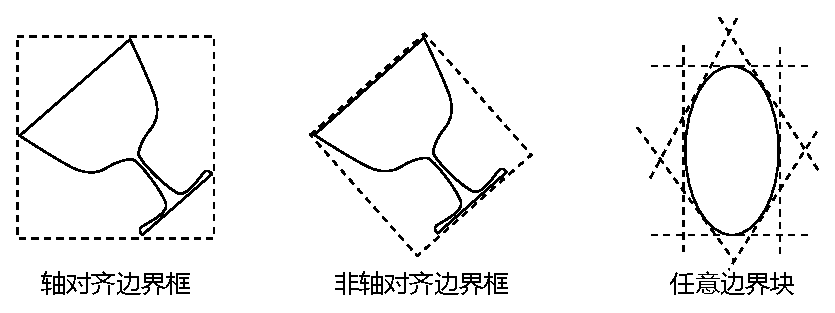
\includegraphics[width=0.8\linewidth]{chap02/Boundingchoices.eps}
          \end{figure}
    \item \circleone 修改pbrt使其像\refvar{Vector3f}{}那样变换\refvar{Normal3f}{},
          并创建因该bug而给出明显错误图像的场景。(完成后别忘了从你的源码拷贝中清除该修改!)
    \item \circletwo 例如,如果一个变换只有平移分量是时变的,则\refvar{AnimatedTransform}{}
          的实现会不必要地计算两个相同旋转之间的插值。修改\refvar{AnimatedTransform}{}
          的实现使其在不需要当前实现中完整一般性的情况下避免这些工作。
          对于适用于你的优化的场景,你观察到了多大的性能变化?
\end{enumerate}

\subsection*{第2题解答}
